\begin{figure}[t]
\centering
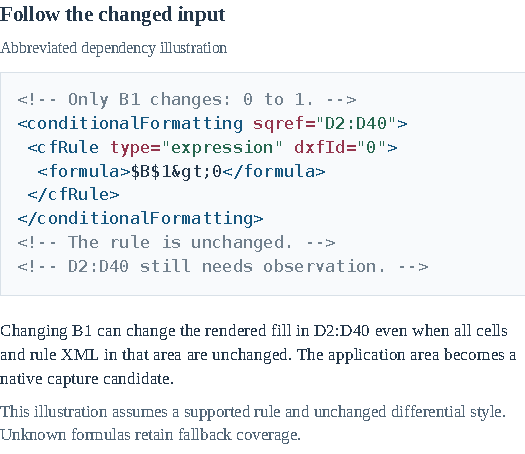
\includegraphics[width=\columnwidth]{figures/capture-methods/05-conditional-input.pdf}
\caption{Changing B1 can change the fill in D2:D40 while its serialized cells
and rule remain unchanged. The application area becomes a native capture
candidate. This example assumes a supported rule and unchanged differential
style. Unknown formulas retain fallback coverage. Abbreviated XML.}
\label{fig:conditional-input}
\end{figure}
